% !TEX root = task-4-5-4.tex
% Editable task bank. Append new BankTask blocks at the end of the document.
\documentclass[12pt,a4paper]{article}
\usepackage{physics-textbook}
\usepackage{graphicx,needspace}
\usetikzlibrary{decorations.pathmorphing}
\newif\ifShowSolutions
\ifdefined\TutorEdition
  \ShowSolutionstrue
\else
  \ShowSolutionsfalse % Change to \ShowSolutionstrue to display solutions.
\fi
\newcounter{banktask}
\newsavebox{\BankTaskBox}
\newcommand{\BankTaskContent}[3]{%
  \noindent\textbf{\thebanktask.}\quad #2\par
  \ifShowSolutions
    \Needspace{50mm}% Keep the solution heading with its opening text or diagram.
    #3\par
    \ifdefined\TutorEdition
      \ifcsname TutorSource#1\endcsname
        \nopagebreak\smallskip{\small\csname TutorSource#1\endcsname\par}%
      \fi
    \fi
  \fi
}
\newcommand{\BankTask}[3]{%
  \refstepcounter{banktask}\par\medskip
  \sbox{\BankTaskBox}{\begin{minipage}{\linewidth}%
    \BankTaskContent{#1}{#2}{#3}\end{minipage}}%
  \ifdim\dimexpr\ht\BankTaskBox+\dp\BankTaskBox\relax>\dimexpr\textheight-20mm\relax
    \Needspace{35mm}\BankTaskContent{#1}{#2}{#3}%
  \else
    \Needspace{\dimexpr\ht\BankTaskBox+\dp\BankTaskBox\relax}%
    \noindent\usebox{\BankTaskBox}\par
  \fi
  \medskip
}
\begin{document}
\BookSubsection{4.5.4}{Ход лучей в собирающей линзе}


% Source 16868: https://phys-ege.sdamgia.ru/problem?id=16868
\BankTask{16868}{
\begin{center}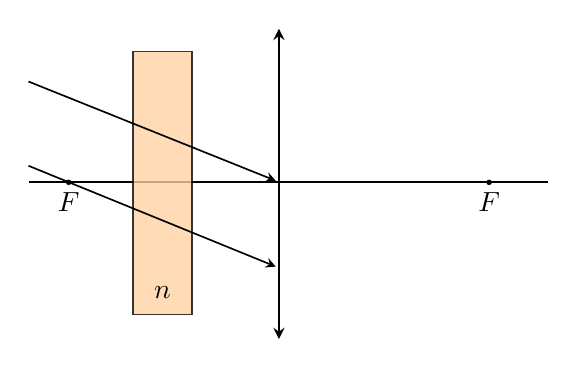
\begin{tikzpicture}[>=stealth,line width=.6pt]

\draw(-3.18,0)--(3.42,0);
\draw[<->,thick](0,-1.99)--(0,1.95);
\fill(-2.67,0)circle(.035) (2.67,0)circle(.035);
\node[below]at(-2.67,0){$F$};\node[below]at(2.67,0){$F$};
\draw[fill=orange!36,opacity=.78](-1.85,-1.68)rectangle(-1.10,1.66);\node at(-1.48,-1.4){$n$};\draw[->](-3.18,1.28)--(-.04,.02);\draw[->](-3.18,.21)--(-.04,-1.07);
\end{tikzpicture}\end{center}
На тонкую собирающую линзу от удаленного источника падает пучок параллельных лучей (см. рис.). Как изменится положение изображения источника, создаваемого линзой, если между линзой и ее фокусом поставить плоскопараллельную стеклянную пластинку с показателем преломления n (на рисунке положение пластинки отмечено пунктиром)? Ответ поясните, указав, какие физические закономерности Вы использовали. Сделайте рисунок, поясняющий ход лучей до и после установки плоскопараллельной стеклянной пластинки.
}{
\smallskip\noindent\textbf{Решение}\par
Построим изображение в линзе до и после установки плоскопараллельной пластинки. Для построения изображения пользуемся следующими соображениями. Луч, проходящий через центр линзы проходит непреломленным. Параллельный пучок света собирается в фокальной плоскости линзы.
После установки плоскопараллельной пластинки луч света будет преломляться внутри нее, но на выходе получим пучок света параллельный исходному. Поясним это соображение. По закону Снеллиуса оптические плотности сред n$_{1}$, n$_{2}$, угол падения $\alpha_{1}$, угол преломления $\alpha_{2}$, связаны соотношением: $n_1 \sin \alpha _1 = n_2 \sin \alpha _2.$ При выходе из пластины закон Снеллиуса также выполняется, получаем: $n_1 \sin \alpha _1 = n_2 \sin \alpha _2 = n_1 \sin \alpha _3.$ То есть синусы падающего и выходящего лучей равны, а значит, равны и углы под которыми, соответственно, падают и выходят эти лучи.


\begin{center}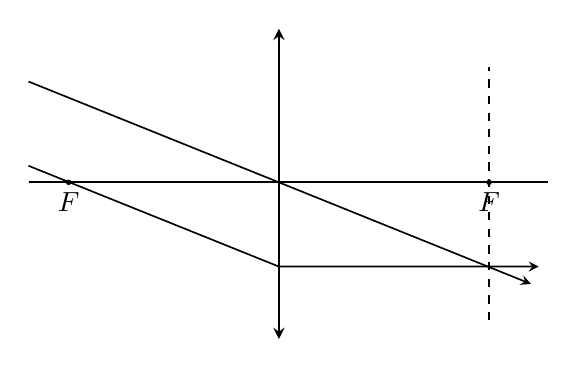
\begin{tikzpicture}[>=stealth,line width=.6pt]

\draw(-3.18,0)--(3.42,0);
\draw[<->,thick](0,-1.99)--(0,1.95);
\fill(-2.67,0)circle(.035) (2.67,0)circle(.035);
\node[below]at(-2.67,0){$F$};\node[below]at(2.67,0){$F$};
\draw[dashed](2.67,-1.75)--(2.67,1.47);\draw[->](-3.18,1.28)--(0,0)--(3.20,-1.29);\draw[->](-3.18,.21)--(0,-1.07)--(3.30,-1.07);
\end{tikzpicture}\end{center}



\begin{center}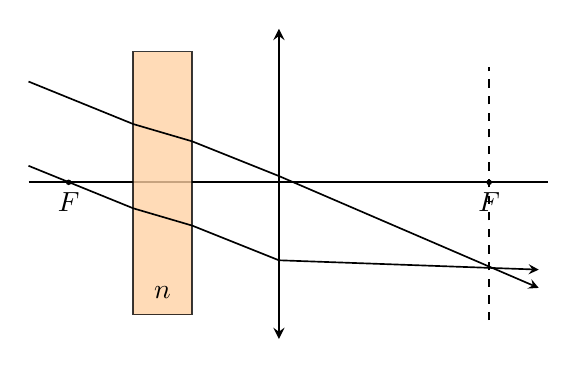
\begin{tikzpicture}[>=stealth,line width=.6pt]

\draw(-3.18,0)--(3.42,0);
\draw[<->,thick](0,-1.99)--(0,1.95);
\fill(-2.67,0)circle(.035) (2.67,0)circle(.035);
\node[below]at(-2.67,0){$F$};\node[below]at(2.67,0){$F$};
\draw[fill=orange!36,opacity=.78](-1.85,-1.68)rectangle(-1.10,1.66);\node at(-1.48,-1.4){$n$};\draw[dashed](2.67,-1.75)--(2.67,1.47);\draw[->](-3.18,1.28)--(-1.85,.74)--(-1.10,.52)--(0,.08)--(3.30,-1.341);\draw[->](-3.18,.21)--(-1.85,-.33)--(-1.10,-.55)--(0,-.99)--(3.30,-1.109);
\end{tikzpicture}\end{center}


Таким образом, получаем, что положение изображения источника после установки плоскопараллельной пластинки не изменится.
}

% Source 43126: https://phys-ege.sdamgia.ru/problem?id=43126
\BankTask{43126}{
К решетке вплотную поставили линзу, которая собирает лучи в одной точке на экране. Линза расположена между решеткой и экраном. Расстояние от линзы до экрана $2\,\text{м}$. Ширина спектра второго порядка $8\,\text{см}$. Длина волны красного света $8$ · $10^{-7}$ и фиолетового света $4$ · $10^{-7}$ м. Найдите, сколько штрихов приходится на $1\,\text{см}$ решетки. $\sin \varphi \approx \tan \varphi \approx \varphi.$
}{
\smallskip\noindent\textbf{Решение}\par
Условие дифракционного максимума $d \sin \varphi =k\lambda,$ где для малых углов $\sin \varphi \approx \tan \varphi = \frac{b}{L} .$
Тогда для максимума фиолетового и красного света получаем

$\frac{db_1}{L} =k\lambda_1$
$\frac{db_2}{L} =k\lambda_2.$

Откуда находим период решетки:

\[d= \frac{Lk ( \lambda_1 - \lambda_2 )}{\Delta b} = \frac{2 \cdot 2 \cdot ( 8 \cdot 10 ^{ - 7 } - 4 \cdot 10 ^{ - 7 } )}{8 \cdot 10 ^{ - 2 }} =2 \cdot 10 ^{ - 5 } \,\text{м}=2 \cdot 10 ^{ - 3 } \,\text{см}.\]

Тогда на $1\,\text{см}$ приходится количество штрихов:

\[N= \frac{1\,\text{см}}{d} = \frac{1}{2 \cdot 10 ^{ - 3 }} =500.\]

Ответ: $500$.
}

% Source 29760: https://phys-ege.sdamgia.ru/problem?id=29760
\BankTask{29760}{
Рассеивающая линза с фокусным расстоянием $F_1=10$ см расположена перед собирающей линзой с фокусными расстоянием $F_2=15$ см. Лучи, идущие от точечного источника света, расположенного на расстоянии $d=10$ см от pacceивающей линзы, пройдя систему образовали пучок лучей, параллельный главной оптической оси. Найдите расстояние между линзами.
}{
\smallskip\noindent\textbf{Решение}\par
$1$.  Найдем расстояние от рассеивающей линзы до изображения точечного источника света по формуле тонкой линзы 

\[\frac{1}{d} - \frac{1}{f} = - \frac{1}{F_1} ,\]

 откуда 

\[f= \frac{d F_1}{d + F_1} = \frac{10 \cdot 10}{10 + 10} =5 \,\text{см}.\]

 Это мнимое изображение находится перед рассеивающей линзой. 
$2$.  Учитывая, что данная точка является источником для собирающей линзы, а лучи после прохождения через нее параллельны, делаем вывод, что эта точка находится в фокусе собирающей линзы, то есть на расстоянии $15\,\text{см}$.
$3$.  Тогда расстояние между линзами равно $x=F_2 - f=15 - 5=10 \,\text{см}.$ 

Ответ: $10\,\text{см}$.
}

\end{document}
